\documentclass[12pt, a4paper]{article}
\usepackage[utf8]{inputenc}
\usepackage{ragged2e}

\usepackage{graphicx, geometry, hyperref, wrapfig, amsmath, subcaption}
\usepackage[dvipsnames]{xcolor}

\definecolor{silver}{RGB}{200,200,200}
\hypersetup{colorlinks=true, linkcolor=RoyalBlue, urlcolor=RoyalBlue}

 \geometry{
 a4paper,
 total={175mm,257mm},
 left=20mm,
 top=15mm,
 }

\usepackage{xcolor} % for defining colour
\usepackage{titlesec} % for customizing sections

% \usepackage{times}        % Use Times New Roman font
% \usepackage{helvet}       % Use Helvetica font
\usepackage{palatino}

\usepackage[T1]{fontenc}

\setlength\parindent{0pt}

% %%%%%%%%%%%%%%%%%%%%%%%%%%%%%%%%%%%%%%%%%%%%%%%%%%%%%%%%%%%%%%
\titleformat{\section}
{\color{UM_DarkBlue}\normalfont\large\bfseries}
{\color{UM_DarkBlue}\thesection}{1em}{}

%%%%%%%%%%%%%%%%%%%%%%%%%%%%%%%%%%%%%%%%%%%%%%%%%%%%%%%%%%%%%%%
\definecolor{UM_Brown}{HTML}{3D190D}
\definecolor{UM_DarkBlue}{HTML}{2264B0}
\definecolor{UM_LightBlue}{HTML}{1CA9E1}
\definecolor{UM_Orange}{HTML}{fEB415}

%%%%%%%%%%%%%%%%%%%%%%%%%%%%%%%%%%%%%%%%%%%%%%%%%%%%%%%%%%%%%%%%

\newcommand{\eg}{{\it e.g.}}
\newcommand{\ie}{{\it i.e.}}

% %%%%%%%%%%%%%%%%%%%%%%%%%%%%%%%%%%%%%%%%%%%%%%%%%%%%%%%%%%%%%%
% \hypersetup{
%     draft=false,
%     final=true,
%     colorlinks=true,
%     citecolor=UM_DarkBlue,
%     anchorcolor=yellow,
%     linkcolor=UM_DarkBlue,
%     urlcolor=UM_DarkBlue,
%     filecolor=green,      
%     pdfpagemode=FullScreen,
%     bookmarksopen=false
%     }
\usepackage{amsmath,amsfonts,amssymb,bm}

%%%%%%%%%%%%%%%%%%%%%%%%%%%%%%%%%%%%%%%%%%%%%%%%%%%%%%%%%%%%%
% Sets and Notations
\newcommand{\reals}{\mathbb{R}}
\newcommand{\integers}{\mathbb{Z}}

%%%%%%%%%%%%%%%%%%%%%%%%%%%%%%%%%%%%%%%%%%%%%%%%%%%%%%%%%%%%%
% Vectors and Matrices
% \renewcommand{\vec}[1]{\bm{\mathrm{#1}}}
\newcommand{\dotp}{\,\boldsymbol{\cdot}\,}
\newcommand{\grad}[1]{\vec{\nabla}#1}
\renewcommand{\div}[1]{\vec{\nabla}\!\dotp\!\vec{#1}}
\newcommand{\curl}[1]{\vec{\nabla}\!\times\!\vec{#1}}



%%%%%%%%%%%%%%%%%%%%%%%%%%%%%%%%%%%%%%%%%%%%%%%%%%%%%%%%%%%%%
% Derivatives
\newcommand{\dv}[2]{\frac{d#1}{d#2}}
\newcommand{\ndv}[3][2]{\frac{d^{\,#1}#2}{d#3^{\,#1}}}

\newcommand{\pdv}[2]{\frac{\partial#1}{\partial#2}}
\newcommand{\npdv}[3][2]{\frac{\partial^{\,#1}#2}{\partial#3^{#1}}}
 
\title{OWO-GAship}
\author{Anik Mandal}
\date{January 2025}
\pagenumbering{arabic}

%====================================================================================================
\begin{document}

\begin{minipage}[t][][c]{0.1\textwidth}
    \begin{flushleft}
        
\includegraphics[height=2cm]{tex-resources/Ashoka Logo.png}
    \end{flushleft}
\end{minipage}
\begin{minipage}[t][][c]{0.85\textwidth}
    \begin{center}
        {\LARGE Oscillations, Wave and Optics}\\ \vspace{0.5em}
        \textsc{(Spring 2025)}\\
        \vspace{1em}
        \textbf{\Large ASSIGNMENT-1} \\
    \end{center}
\end{minipage}
\vspace{10pt}\\
\rule[0em]{\textwidth}{0.75pt}

\flushleft{Topics: SHO, Damped and Driven Harmonic Oscillation \hfill
Total : 40 \\
\flushleft{Date: 3th Feb, 2025}\hfill
\fbox{\textbf{\large 
Due: 16th Feb, 2025} (EoD)}\\
\vspace{.2cm}
\rule[0em]{\textwidth}{1.75pt}
\vspace{-1cm}

%====================================================================================================
%====================================================================================================
\justifying

\section*{Part:A \hfill \textbf{[20]}}

\textbf{(i)} A small body rests on a horizontal diaphragm of 
a loudspeaker that is supplied with an alternating current of
constant amplitude but variable frequency. If the diaphragm executes
simple harmonic oscillation in the vertical direction of amplitude $10\mu m$,
at all frequencies, find the greatest frequency (in hertz) for which 
the small body stays in contact with the diaphragm. [Figure-\ref{fig:speaker}][\textit{Hint: 
Try to find the expression for normal force(N), find the condition for N=0}]
\hfill \textbf{2}\\
\begin{figure*}[h]
    \begin{subfigure}{.35\textwidth}
        \centering
        \includegraphics*[scale=0.2]{figs/speaker.jpeg}
        \caption{}
        \label{fig:speaker}
    \end{subfigure}
    \begin{subfigure}{.2\textwidth}
        \centering
        \includegraphics*[scale=0.14]{figs/Utube.jpeg}
        \caption{}
        \label{fig:U-tube}
    \end{subfigure}
    \begin{subfigure}{.52\textwidth}
        \centering
        \includegraphics*[scale=0.16]{figs/semi-cir-depression.jpeg}
        \caption{}
        \label{fig:semi-circ-depression}
    \end{subfigure}
\end{figure*}

\noindent
\textbf{(ii)} A U-tube of constant cross-sectional area $A$ consists of a horizontal section 
connected at either end to two vertical sections. Suppose that the tube is filled with an 
incompressible liquid of mass density $\rho$. Let the total length of the liquid column be $l$. 
(Where $l$ exceeds the length of the horizontal section.) Suppose that the surface of the liquid 
in one of the vertical sections is initially displaced (vertically) a small distance $h$ from its 
equilibrium position. Show that the surface displacement subsequently executes simple harmonic 
oscillation at the angular frequency $\omega=\sqrt{2\,g/l}$, where $g$ is the acceleration due to 
gravity. [Figure-\ref{fig:U-tube}][\textit{Hint: Try to find the expression for restoring force.}]
\hfill \textbf{3}\\

\noindent
\textbf{(iii)} A particle of mass $m$ slides in a frictionless semi-circular depression in the 
ground of radius $R$. Find the angular frequency of small amplitude oscillations about the 
particle's equilibrium position, assuming that the oscillations are essentially one-dimensional, 
so that the particle passes through the lowest point of the depression during each oscillation cycle.
[Figure-\ref{fig:semi-circ-depression}][\textit{Hint: Try to find the expression for restoring force.}]
\hfill \textbf{3}\\


\noindent
\textbf{(iv)}Show that the average speed of a particle executing simple harmonic oscillation is $2/\pi$ 
times the maximum speed. [\textit{Hint: You know the difference between speed and velocity, just take the average.}]
\hfill \textbf{3}\\

\noindent
\textbf{(v)} A compound pendulum consists of a uniform bar of length $l$ that pivots about one of its 
ends. Show that the pendulum has the same period of oscillation as a simple pendulum of length 
$(2/3)l$. [Figure-\ref{fig:compound-pend}][\textit{Hint: Derive the expression for restoring torque and 
calculate moment of inertia}] \hfill \textbf{3}\\ \\
\begin{figure*}[t]
    \begin{subfigure}{.5\textwidth}
        \centering
        \includegraphics*[scale=0.1]{figs/compound-pend.jpeg}
        \caption{}
        \label{fig:compound-pend}
    \end{subfigure}
    \begin{subfigure}{.2\textwidth}
        \centering
        \includegraphics*[scale=0.13]{figs/LC-circuit.jpeg}
        \caption{}
        \label{fig:LC-circuit}
    \end{subfigure}
\end{figure*}
\noindent
\textbf{(vi)} Show that the ratio of two successive maxima in the displacement of a damped harmonic
oscillator is constant.[\textit{Hint: For a given solution x(t) find the locations of maxima, calculate x(t) 
at those locations.}]
\hfill \textbf{2}\\

\noindent
\textbf{(vii)} An LC circuit is such that at $t=0$ the capacitor is uncharged and a current $I_0$ flows through 
the inductor. Find an expression for the charge $Q$ stored on the positive plate of the capacitor 
as a function of time.[Figure-\ref{fig:LC-circuit}] [\textit{Hint : You have to find Q(t) from I(t) or you can 
solve ODE for Q(t) and find I(t) then apply BCs}]\hfill \textbf{4}\\


\section*{Part:B \hfill \textbf{[20]}}
\textbf{(i)} A particle of mass $m$ executes one-dimensional simple harmonic oscillation such 
that its instantaneous $x$ coordinate is

\begin{align*}
    x(t) = a \cos(\omega t-\phi)
\end{align*}
(a) Find the average values of $x$, $x^2$, $\dot{x}$, and $\dot{x}^2$ over a single cycle of the oscillation.\\
(b) Find the average values of the kinetic and potential energies of the particle over a single cycle of 
the oscillation. [\textit{Hint: Take the single cycle from t= $\phi/\omega$  to $(\phi  + 2\pi)/\omega$}] 
\hfill \textbf{2+2}\\

\noindent
\textbf{(ii)} A particle executing simple harmonic oscillation in one dimension has speeds $u$ and $v$
at displacements $a$ and $b$, respectively, from its equilibrium position.
Show that the period of the motion can be written
\begin{align*}
    T = 2\pi\left(\frac{b^2-a^2}{u^2-v^2}\right)^{1/2}
\end{align*}

Show that the amplitude of the motion can be written

\begin{align*}
    A= \left(\frac{u^2 b^2-v^2 a^2}{u^2-v^2}\right)^{1/2}
\end{align*}[\textit{Hint: Derive the expression for v(t) as a function of x(t) or find v(x)}]  \hfill \textbf{2+2}\\

\noindent
\textbf{(iii)} Imagine a straight tunnel passing through the center of the Earth, which is regarded 
as a sphere of radius $R$ and uniform mass density. A particle is dropped into the tunnel from the 
surface. Show that the particle undergoes simple harmonic oscillation at the angular frequency 
$\omega=\sqrt{g/R}$, where $g$ is the gravitational acceleration at Earth's surface. (Hint: The 
gravitational acceleration at a point inside a spherically symmetric mass distribution is the same 
as if all of the mass interior to the point were concentrated at the center, and all of the mass 
exterior to the point were neglected.) Estimate how long it takes the particle to reach the other 
end of the tunnel.

Assuming that the tunnel is smooth (i.e., ignoring friction), show that motion is simple harmonic 
even if the tunnel does not pass through the center of the Earth, and that the travel time from one 
end of the tunnel to the other is the same as before.[Figure-\ref{fig:tunnel-through-earth}][\textit{Hint: 
Try to find the expression for restoring force.}] \hfill \textbf{2+2}\\
\begin{figure*}[h]
    \centering
    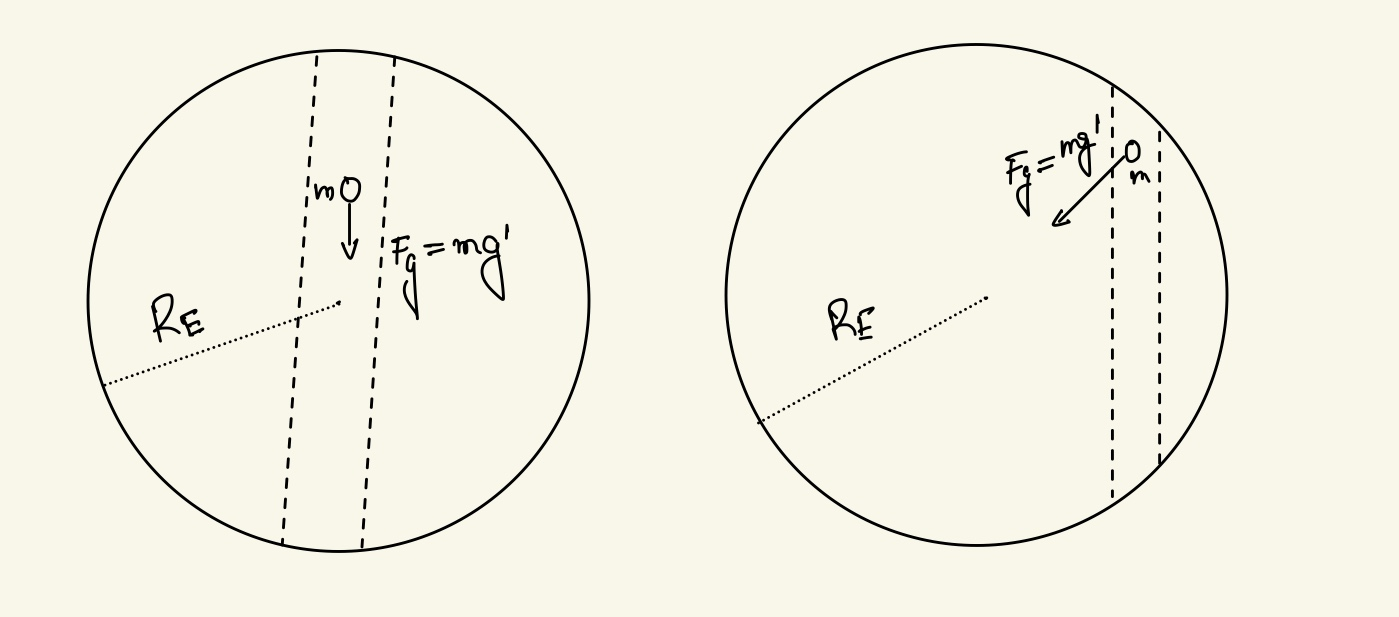
\includegraphics[scale=0.2]{figs/tunnel-through-earth.jpeg}
    \caption{}
    \label{fig:tunnel-through-earth}
\end{figure*}

\noindent
\textbf{(iv)} According to classical electromagnetic theory, an accelerated electron radiates energy 
at the rate $K e^2 a^2 /c^3$, where $K=6\times 10^9 \rm N m^2 / \rm C^2,  e$ is the 
charge on an electron, $a$ the instantaneous acceleration, and $c$ the velocity of light in vacuum.

(a)If an electron were oscillating in a straight line with displacement $x(t)= A \sin(2\pi ft)$, 
how much energy would it radiate away during a single cycle?

(b)What is the effective $Q_f$ of this oscillator?

(c)How many periods of oscillation would elapse before the energy of the oscillation was reduced 
to half of its initial value?

(d)Substituting a typical optical frequency (e.g., for green light) for $f$, give numerical estimates 
for the $Q_f$ and half-life of the radiating system.
[\textit{Hint: (b) Use the definition of $Q_f$. (c) Try to find the expression of E(t)}] \hfill \textbf{8}\\


\end{document}